\documentclass[9pt,twocolumn,twoside,]{pnas-new}

% Use the lineno option to display guide line numbers if required.
% Note that the use of elements such as single-column equations
% may affect the guide line number alignment.


\usepackage[T1]{fontenc}
\usepackage[utf8]{inputenc}

% tightlist command for lists without linebreak
\providecommand{\tightlist}{%
  \setlength{\itemsep}{0pt}\setlength{\parskip}{0pt}}


% Pandoc citation processing
%From Pandoc 3.1.8
% definitions for citeproc citations
\NewDocumentCommand\citeproctext{}{}
\NewDocumentCommand\citeproc{mm}{%
  \begingroup\def\citeproctext{#2}\cite{#1}\endgroup}
\makeatletter
 % allow citations to break across lines
 \let\@cite@ofmt\@firstofone
 % avoid brackets around text for \cite:
 \def\@biblabel#1{}
 \def\@cite#1#2{{#1\if@tempswa , #2\fi}}
\makeatother
\newlength{\cslhangindent}
\setlength{\cslhangindent}{1.5em}
\newlength{\csllabelwidth}
\setlength{\csllabelwidth}{3em}
\newenvironment{CSLReferences}[2] % #1 hanging-indent, #2 entry-spacing
 {\begin{list}{}{%
  \setlength{\itemindent}{0pt}
  \setlength{\leftmargin}{0pt}
  \setlength{\parsep}{0pt}
  % turn on hanging indent if param 1 is 1
  \ifodd #1
   \setlength{\leftmargin}{\cslhangindent}
   \setlength{\itemindent}{-1\cslhangindent}
  \fi
  % set entry spacing
  \setlength{\itemsep}{#2\baselineskip}}}
 {\end{list}}
\usepackage{calc}
\newcommand{\CSLBlock}[1]{#1\hfill\break}
\newcommand{\CSLLeftMargin}[1]{\parbox[t]{\csllabelwidth}{#1}}
\newcommand{\CSLRightInline}[1]{\parbox[t]{\linewidth - \csllabelwidth}{#1}\break}
\newcommand{\CSLIndent}[1]{\hspace{\cslhangindent}#1}

\providecommand{\pandocbounded}[1]{#1}
\usepackage{booktabs}
\usepackage{float}
\usepackage{graphicx}
\usepackage{amsmath}
\usepackage{amsfonts}
\usepackage{amssymb}
\usepackage{bbm}
\usepackage{algorithm}
\usepackage{algpseudocode}
\usepackage{setspace}
\DeclareMathOperator*{\argmin}{argmin}
\DeclareMathOperator*{\argmax}{argmax}
\DeclareMathOperator\diag{diag}
\renewcommand{\algorithmicrequire}{\textbf{Input:}}
\renewcommand{\algorithmicensure}{\textbf{Output:}}

\templatetype{pnasresearcharticle}  % Choose template

\title{Survival driven deconvolution (deSurv) reveals prognostic and
interpretable cancer subtypes}

\author[a,1,2]{Amber M. Young}
\author[b]{Alisa Yurovsky}
\author[a]{Didong Li}
\author[a,c]{Naim U. Rashid}

  \affil[a]{University of North Carolina at Chapel Hill, Biostatistics,
Street, City, State, Zip}
  \affil[b]{Stony Brook University, Street, City, State, Zip}


% Please give the surname of the lead author for the running footer
\leadauthor{Anonymous}

% Please add here a significance statement to explain the relevance of your work
\significancestatement{Understanding which molecular programs influence
patient survival remains a central challenge in cancer genomics. We
developed DeSurv, a survival-driven deconvolution framework that
integrates nonnegative matrix factorization with Cox regression to
identify latent gene-expression programs directly linked to clinical
outcomes. Applied to pancreatic ductal adenocarcinoma, DeSurv uncovered
interpretable tumor and stromal factors that generalize across
independent cohorts and align with established subtypes. By coupling
survival modeling with matrix factorization, DeSurv bridges the gap
between biologically descriptive and prognostically relevant signatures,
revealing that patient outcomes are shaped by the combined activity of
basal and immune-stromal programs. This approach provides a broadly
applicable strategy for discovering outcome-associated transcriptional
programs in complex cancers.}


\authorcontributions{Please provide details of author contributions
here.}

\authordeclaration{Please declare any conflict of interest here.}


\correspondingauthor{\textsuperscript{2} To whom correspondence should
be addressed. E-mail:
\href{mailto:ayoung31@live.unc.edu}{\nolinkurl{ayoung31@live.unc.edu}}}

% Keywords are not mandatory, but authors are strongly encouraged to provide them. If provided, please include two to five keywords, separated by the pipe symbol, e.g:
 \keywords{  one |  two |  optional |  optional |  optional  } 

\begin{abstract}
Molecular subtyping in cancer is an ongoing problem that relies on the
identification of robust and replicable gene signatures. While
transcriptomic profiling has revealed recurrent gene expression patterns
in various types of cancer, the prognostic value of these signatures is
typically evaluated in retrospect. This is due to the reliance on
unsupervised learning methods for identifying cell-type-specific signals
and clustering patients into molecular subtypes. Here we present a
Survival-driven Deconvolution tool (deSurv) that integrates bulk
RNA-sequencing data with patient survival information to identify
cell-type-enriched gene signatures associated with prognosis. Applying
deSurv to various cohorts in pancreatic cancer, we uncover prognostic
and biologically interpretable subtypes that reflect the complex
interactions between stroma, tumor, and immune cells in the tumor
microenvironment. Our approach highlights the value of using patient
outcomes during gene signature discovery.
\end{abstract}

\dates{This manuscript was compiled on \today}
\doi{\url{www.pnas.org/cgi/doi/10.1073/pnas.XXXXXXXXXX}}

\begin{document}

% Optional adjustment to line up main text (after abstract) of first page with line numbers, when using both lineno and twocolumn options.
% You should only change this length when you've finalised the article contents.
\verticaladjustment{-2pt}



\maketitle
\thispagestyle{firststyle}
\ifthenelse{\boolean{shortarticle}}{\ifthenelse{\boolean{singlecolumn}}{\abscontentformatted}{\abscontent}}{}

% If your first paragraph (i.e. with the \dropcap) contains a list environment (quote, quotation, theorem, definition, enumerate, itemize...), the line after the list may have some extra indentation. If this is the case, add \parshape=0 to the end of the list environment.

\acknow{Please include your acknowledgments here, set in a single
paragraph. Please do not include any acknowledgments in the Supporting
Information, or anywhere else in the manuscript.}

Molecular subtyping has become a cornerstone of precision oncology,
enabling the classification of patients into biologically distinct
groups that inform prognosis and guide therapeutic decisions (1--5).
Defining these subtypes depends on identifying robust genomic or
transcriptomic signatures that capture the molecular programs driving
disease heterogeneity (6--9).

However, tumors are composed of diverse cell types---including
malignant, stromal, immune, and endothelial populations---whose
gene-expression signals are deeply interwoven. This complexity makes it
difficult to isolate the signatures that truly characterize each subtype
or to distinguish tumor-intrinsic programs from those shaped by the
surrounding microenvironment. Furthermore, some molecular programs may
delineate distinct aspects of tumor biology but not demonstrate clinical
relevance with respect to patient outcomes (10--12). This disconnect
highlights a key challenge in translational genomics: distinguishing the
molecular features that merely describe tumor heterogeneity from those
that are predictive of disease course or therapeutic response.

Single-cell transcriptomic technologies have transformed our
understanding of tumor ecosystems by resolving the diversity of cell
types and states within the tumor microenvironment (13). Yet their high
cost and limited cohort sizes often preclude systematic evaluation of
clinical outcomes, so the molecular programs they uncover are typically
assessed downstream in bulk datasets for prognostic or therapeutic
relevance. Bulk transcriptomic studies---while lacking cellular
resolution---have been conducted across many independent patient
cohorts, which collectively encompass hundreds to thousands of
clinically annotated samples (14, 15). These datasets provide the
statistical power to evaluate molecular programs in relation to patient
outcomes, highlighting a trade-off between biological resolution and
clinical scalability.

To address the limited resolution of bulk data, numerous computational
deconvolution approaches have been developed to infer the relative
abundance of distinct cell types and their gene-expression programs,
summarized in this review (16). These methods often rely on reference
signatures derived from sorted or single-cell data to estimate cellular
composition and attribute gene-expression patterns to known cell types.
While such approaches have been valuable for characterizing the tumor
microenvironment, they depend on predefined references and therefore
cannot discover new or context-specific molecular programs.

Unsupervised matrix factorization methods, particularly Nonnegative
Matrix Factorization (NMF) (17), have been instrumental in revealing
latent molecular programs that define tumor heterogeneity, especially in
pancreatic cancer (18--21). NMF excels at identifying biologically
meaningful patterns in gene-expression data (22) but is limited in
prognostic ability due to its unsupervised nature (23). Additionally,
the non-uniqueness of NMF solutions can make replicability across
studies challenging. Consequently, the uncovered programs frequently
capture broad biological variation, such as cell type composition,
rather than the specific molecular features that influence prognosis or
treatment response.

To bridge this gap, we introduce DeSurv, a semi-supervised deconvolution
framework that integrates NMF with the Cox proportional hazards model
(24). By integrating survival modeling directly into the matrix
factorization framework, DeSurv learns de novo molecular programs that
are both biologically interpretable and prognostic of patient outcomes.
Importantly, DeSurv incorporates an automated cross-validation framework
to determine key parameters, including the optimal number of latent
factors---addressing a major limitation of fully unsupervised approaches
that rely on heuristic or subjective choices. Applied to pancreatic
adenocarcinoma (PDAC) data, DeSurv uncovered molecular programs
representing blended tumor, stromal, and immune features, suggesting
that integrating survival information can reveal novel prognostic
interactions between tumor and microenvironmental processes.

\section*{Results}\label{results}
\addcontentsline{toc}{section}{Results}

\subsection*{Model Overview}\label{model-overview}
\addcontentsline{toc}{subsection}{Model Overview}

We have developed an integrated framework, DeSurv, that couples
Nonnegative Matrix Factorization (NMF) with Cox proportional hazards
regression to identify latent gene-expression programs associated with
patient survival (Fig. 1). The model takes as input a bulk expression
matrix of \(p\) genes by \(n\) patients (\(X_{Train}\)) together with
corresponding survival times (\(y_{Train}\)) and censoring indicators
(\(\delta_{Train}\)) (Fig. 1A).

DeSurv optimizes a joint objective combining the NMF reconstruction loss
and the Cox model's log-partial likelihood, weighted by a supervision
parameter (\(\alpha\)) that determines the relative contribution of each
term (Fig. 1B): \begin{align}
  (1-\alpha)\ &\mathcal{L}_{NMF}(X_{Train} \approx WH)\nonumber \\ - \alpha\ &\mathcal{L}_{Cox}(X_{Train}^TW\beta,y_{Train},\delta_{Train})
\end{align} When \(\alpha=0\), the method reduces to standard
unsupervised NMF; when \(\alpha>0\), survival information directly
guides the learned factors toward prognostic structure.

Within this framework, the product (\(X_{Train}^TW\)) represents
patient-level factor scores - the inferred burden of each latent program
across subjects. These factor scores serve as covariates in the Cox
model, and their regression coefficients (\(\beta\)) indicate whether
higher activity of a given program corresponds to improved or reduced
survival.

Model training yields gene weights (\(\hat{W}\)), factor loadings
(\(\hat{H}\)), and Cox coefficients (\(\hat{\beta}\)) (Fig. 1C), where
the inner dimension (\(k\)) specifies the number of latent factors.
Genes with high gene weights in one factor and low gene weights in all
others define the factor-specific signature genes (Fig. 1D). By
integrating survival supervision into the factorization, DeSurv not only
reconstructs the underlying expression structure, preserving biologial
interpretability, but also guides latent factors to be prognostically
informative. Subsequent analyses can therefore focus on the
survival-associated gene programs (Fig. 1E).

\begin{figure*}[t]

{\centering \includegraphics[width=\textwidth,height=4in]{../figures/model_schematic_training} 

}

\caption{DeSurv overview. Overview of the DeSurv training pipeline. A. The input is a preprocessed bulk gene expression matrix and patient survival outcomes. B. The Desurv model optimizes a joint NMF + Cox loss function. C. The DeSurv model estimates three quantities: Gene weights matrix (W), Subject loadings matrix (H), and regression coefficients from the Cox model (beta). D. We extract the exemplar genes from each signature in the gene weights matrix. E. The exemplar genes from survival associated factors provide prognostic gene signatures.}\label{fig:fig-schema}
\end{figure*}

\subsection*{\texorpdfstring{The DeSurv pipeline provides an automated
method for choosing the NMF rank (\(k\)) and supervision parameter
(\(\alpha\))}{The DeSurv pipeline provides an automated method for choosing the NMF rank (k) and supervision parameter (\textbackslash alpha)}}\label{the-desurv-pipeline-provides-an-automated-method-for-choosing-the-nmf-rank-k-and-supervision-parameter-alpha}
\addcontentsline{toc}{subsection}{The DeSurv pipeline provides an
automated method for choosing the NMF rank (\(k\)) and supervision
parameter (\(\alpha\))}

We implemented a five-fold cross-validation procedure to identify the
optimal hyperparameters for the DeSurv model---namely, the number of
latent factors (\(k\)) and the supervision strength (\(\alpha\)). In
each fold, the gene-expression matrix and corresponding survival
outcomes were partitioned into training and test sets at the patient
level (Fig. 2A). The DeSurv model was applied to the training set to
estimate the gene weights (\(\hat{W}\)) and regression coefficients
(\(\hat{\beta}\)) (Fig. 2B). The expression matrix for the test set
(\(X_{Test}\)) was projected onto the learned basis (\(\hat{W}\)) to
obtain patient-level factor scores. These scores were multiplied by
regression coefficients (\(\hat{\beta}\)) to generate the linear
predictor for each patient (Fig. 2C), which was then compared against
the true survival outcomes to assess predictive performance (Fig. 2D).

We evaluated the cross-validated concordance index (C-index) across a
grid of model ranks (\(k=\{2, \dots,12\}\)) and supervision parameters
(\(\alpha=\{0, 0.05, 0.10, \dots, 1\}\)) (Fig. 2E). To reduce
overfitting, we selected the smallest combination of \(\alpha\) and
\(k\) within one standard error of the maximum cross validated c-index.
The cross-validated C-index varied modestly across the parameter space,
but models with \(\alpha>0\) consistently outperformed the unsupervised
baseline (\(\alpha=0\)). For each value of \(k\), there existed at least
one \(\alpha>0\) yielding higher predictive accuracy than the
unsupervised equivalent, indicating that incorporating survival
information improves predictive performance. Interestingly, the
supervised models achieved their best performance at smaller values of
\(k\) compared with unsupervised NMF, suggesting that survival-guided
factorization produces a more parsimonious yet more prognostic
representation.

For comparison, we also evaluated standard NMF using the NMF R package,
which lacks an objective means for cross-validation. Conventional
selection of the factor rank \(k\) relies on heuristic metrics such as
cophenetic correlation, dispersion, residual error, explained variance,
silhouette score, and matrix sparseness (Fig. 2F). In our analysis,
cophenetic correlation and dispersion peaked at \(k=3\) and declined
thereafter, indicating reduced clustering stability at higher ranks. In
contrast, explained variance and reconstruction residuals plateaued
around \(k=7\), suggesting that at least this many factors are needed to
adequately reconstruct the expression matrix. The silhouette score was
highest at \(k=2-3\), implying better cluster separation at smaller
ranks, whereas the sparsity of \(W\) and \(H\) was most balanced near
\(k=7\), favoring interpretability at moderate rank. These criteria
therefore yield conflicting recommendations: stability metrics favor
smaller \(k\), while reconstruction and interpretability metrics favor
moderate \(k\). In the cross validation at \(\alpha=0\), survival
prediction under unsupervised NMF did not improve appreciably until
\(k \geq 5\) and peaked at \(k=6\).

In contrast, DeSurv's joint optimization identifies a simpler model
(\(k=3\) and \(\alpha=0.7\)) that achieves superior prognostic
performance compared to standard NMF with a more parsimonious model,
underscoring the advantage of integrating survival supervision into the
matrix factorization process.

\begin{figure*}[t]

{\centering \includegraphics[width=\textwidth,height=5.5in]{/work/users/a/y/ayoung31/DeSurv-paper/paper/paper_ntop=50_ngene=2000_files/figure-latex/fig-cv-1} 

}

\caption{A. Overview of DeSurv cross-validation pipeline. B. Heatmap of cross-validated C-index with columns k and rows alpha. C. Plots of various metrics used to choose k in the standard NMF setting.}\label{fig:fig-cv}
\end{figure*}

\subsection*{DeSurv provides biologically interpretable gene
signatures}\label{desurv-provides-biologically-interpretable-gene-signatures}
\addcontentsline{toc}{subsection}{DeSurv provides biologically
interpretable gene signatures}

For the selected DeSurv model (\(k=3, \alpha=0.7\)), we identified the
top 50 factor-specific genes from each latent factor to characterize
their underlying biological functions. Figures 3A--C summarize the
results of an over-representation analysis (ORA) performed on these
genes. The enrichment profiles reveal three distinct biological
programs. Factor 1 is strongly enriched for immune-related pathways,
including cytokine signaling, T-cell activation, and interferon
response. Factor 2 shows enrichment for genes associated with normal
pancreatic or exocrine function, suggesting that this component captures
residual normal-tissue signal. Factor 3 is enriched for pathways linked
to epithelial--mesenchymal transition, cell cycle progression, and KRAS
signaling---features typically associated with the Basal-like subtype of
pancreatic ductal adenocarcinoma (PDAC).

Survival analysis of the factor signature scores on the training data
demonstrates clear prognostic stratification. High expression of Factor
1 is associated with longer overall survival (HR = 0.37, p \textless{}
2e-16), whereas Factor 3 is linked to significantly shorter survival (HR
= 1.43, p = 2e-4). These trends are consistent with known biology:
immune-infiltrated tumors generally exhibit improved prognosis, while
Basal-like tumors are aggressive and clinically refractory. Factor 2,
corresponding to the normal/exocrine signal, shows no significant
association with survival (HR = 0.99, p = 0.91), indicating that while
this component contributes to reconstructing the expression matrix, it
does not carry prognostic information. This behavior illustrates a key
property of DeSurv---its joint optimization ensures that the latent
factors balance both survival relevance and expression reconstruction,
preserving biologically necessary structure even when not directly
linked to outcome.

Figure 3D further examines the correlation between DeSurv factors and
previously published PDAC gene signatures. Factor 1 aligns with
signatures from classical tumor, iCAF and restCAF stroma, and immune
infiltration, all of which are associated with favorable prognosis. In
contrast, Factor 3 correlates with Basal-like tumor, proCAF, and
activated stromal programs, which are generally linked to poor outcomes.
These overlaps suggest that each factor represents a composite axis of
tumor--stroma-immune interaction, capturing biologically coherent
programs that align with known PDAC ecosystems but arise de novo from
the DeSurv model.

\begin{figure*}[t]

{\centering \includegraphics[width=\textwidth,height=4.5in]{/work/users/a/y/ayoung31/DeSurv-paper/paper/paper_ntop=50_ngene=2000_files/figure-latex/fig-bio-1} 

}

\caption{A-C. Dotplots of ORA analysis of top 50 genes from each DeSurv derived factor. D. Correlation between the DeSurv gene weights matrix and previously published PDAC gene signatures.}\label{fig:fig-bio}
\end{figure*}

\subsection*{Clustering patients from external cohorts on DeSurv gene
signatures produces prognostic
subtypes}\label{clustering-patients-from-external-cohorts-on-desurv-gene-signatures-produces-prognostic-subtypes}
\addcontentsline{toc}{subsection}{Clustering patients from external
cohorts on DeSurv gene signatures produces prognostic subtypes}

To evaluate the generalizability of DeSurv-derived prognostic
signatures, we applied the exemplar genes from the survival-associated
factors in the trained model (Factors 1 and 3) to multiple independent
PDAC cohorts---including Dijk, PACA-AU (RNA-seq and microarray),
Moffitt, and Puleo datasets---using their bulk gene-expression profiles.
Unsupervised consensus clustering was performed on each cohort based on
the expression of these prognostic genes. Three clusters were selected
as the optimal solution, supported by inspection of the cumulative
distribution function (CDF) plots, relative change in area under the CDF
curve, consensus heatmaps, and cluster consensus scores (Fig. SX).
Importantly, the number of clusters was determined without incorporating
any survival information, ensuring an unbiased evaluation of downstream
prognostic performance.

Expression heatmaps of the DeSurv prognostic signatures revealed three
distinct transcriptional patterns across the external cohorts (Fig. 4A).
Cluster 1 displayed high expression of the basal-like (Factor 3) gene
set; Cluster 2 showed elevated expression of the immune/iCAF (Factor 1)
signature and reduced basal activity; and Cluster 3 exhibited
intermediate expression of both programs. These patterns suggest that
survival prediction is primarily driven by the presence or absence of
basal and immune/iCAF programs, rather than by a reciprocal contrast
between basal versus classical tumor states or iCAF versus myCAF stromal
signatures.

Additionally, DeSurv-derived clusters showed strong correspondence with
established molecular classifiers. Column annotations in Fig. 4A and the
contingency table in Fig. 4B demonstrate substantial overlap with PurIST
and DeCAF subtype labels: for example, X\% of patients in Cluster 1 were
classified as PurIST Basal-like and DeCAF proCAF, X\% of Cluster 2 as
Classical + restCAF, and X\% of Cluster 3 as Classical + proCAF. The
rarity of the Basal + restCAF subtype likely contributes to the
discovery of 3 rather than 4 clusters. A chi-squared test confirmed a
significant association between the DeSurv-defined clusters and existing
classifier labels (\(\chi^2\) = 210.16 p \textless{} 2.2e-16).

We next assessed the prognostic relevance of these clusters using
overall survival data from the external cohorts (Fig. XC--D). Because
DeSurv was trained exclusively on the TCGA-PAAD and CPTAC
datasets---without access to the expression or outcome data of the
external cohorts---this analysis represents an independent validation of
the model's predictive generalizability. Kaplan--Meier analysis
demonstrated that the DeSurv-derived clusters were strongly associated
with survival (p = 4.8e-6). As expected, the Basal-like cluster (Cluster
1) was associated with the poorest survival, the Classical + restCAF
cluster (Cluster 2) exhibited the most favorable outcomes, and the
Classical + proCAF cluster (Cluster 3) showed intermediate survival.
This pattern mirrors previous findings describing the interplay between
tumor-intrinsic and stromal subtypes in PDAC (e.g., (25)), supporting
the robustness and biological validity of the DeSurv-derived signatures.

\begin{figure*}[t]

{\centering \includegraphics[width=\textwidth,height=4in]{/work/users/a/y/ayoung31/DeSurv-paper/paper/paper_ntop=50_ngene=2000_files/figure-latex/fig-clus-1} 

}

\caption{External cohort validation. A. Heatmap of expression values for genes in the DeSurv factor signatures in external cohorts. B. Table of DeSurv derived clusters by PurIST + DeCAF classifier subtypes in external cohorts. C. Kaplan Meier curves describing survival outcomes for patients from external cohorts in each of the DeSurv derived clusters.}\label{fig:fig-clus}
\end{figure*}

\subsection*{Analysis of scRNA-seq}\label{analysis-of-scrna-seq}
\addcontentsline{toc}{subsection}{Analysis of scRNA-seq}

Next, we verify our findings at the cellular level using the Elyada
scRNA-seq data (cite data). We found that our DeSurv factor 1 signature
was expressed primarily in iCAF and B cells, factor 2 was expressed in
Acinar and Classical PDAC 2, and factor 3 was expressed primarily in
Basal-like PDAC cells (Figures 4B-E). This is consistent with our ORA
analysis which found that factor 1 was mostly immune and factor 3 was
basal-like, and with the overlap we saw with published gene lists that
identified factor 1 as iCAF/classical/immune and factor 3 as basal-like.
Interestingly, we do not see a large overlap of factor 1 with the
classical PDAC cell types despite some overlap with classical gene
lists. Need more here\ldots{}

\begin{figure*}[t]

{\centering 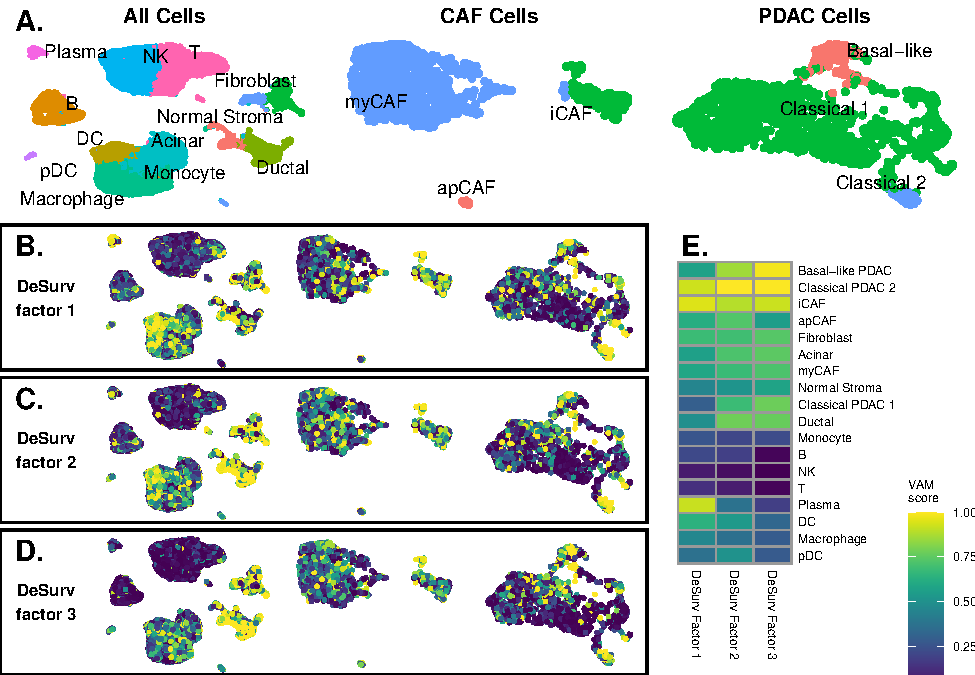
\includegraphics[width=\textwidth,height=8in]{/work/users/a/y/ayoung31/DeSurv-paper/paper/paper_ntop=50_ngene=2000_files/figure-latex/fig-sc-1} 

}

\caption{A. Cell type clusters from the Elyada scRNA-seq data. B-D. VAM scores for the DeSurv factor signatures in each cell shown on the UMAP of cells in the Elyada-sc data. E. Heatmap of average VAM scores by cell type and factor signature in the Elyada-sc data.}\label{fig:fig-sc}
\end{figure*}

\section*{Discussion}\label{discussion}
\addcontentsline{toc}{section}{Discussion}

We present DeSurv, a survival-driven deconvolution framework that
integrates nonnegative matrix factorization with Cox proportional
hazards modeling to uncover latent gene-expression programs associated
with patient outcomes. By coupling unsupervised matrix decomposition
with direct survival supervision, DeSurv bridges the gap between
descriptive molecular subtyping and prognostic modeling. Unlike
conventional NMF, which identifies factors that explain transcriptional
variance without regard to clinical relevance, DeSurv simultaneously
optimizes reconstruction fidelity and survival discrimination, yielding
interpretable gene programs that are both biologically coherent and
clinically informative.

In pancreatic ductal adenocarcinoma (PDAC), DeSurv identified three
major transcriptional programs corresponding to immune/iCAF,
normal/exocrine, and basal-like factors. The immune/iCAF factor was
associated with prolonged survival and enriched for inflammatory and
immune-response pathways, consistent with prior evidence linking
tumor-infiltrating immune and inflammatory fibroblast populations to
improved outcomes. In contrast, the basal-like factor was strongly
associated with poor survival and enriched for epithelial--mesenchymal
transition and cell-cycle programs characteristic of aggressive tumor
phenotypes. The normal/exocrine factor, while not prognostic, captured
background pancreatic tissue signal and contributed to accurate
reconstruction, demonstrating that DeSurv can disentangle prognostic
sources of variation while preserving biology.

Importantly, DeSurv outperformed unsupervised NMF in cross-validated
concordance index, achieving higher predictive accuracy with fewer
factors. This suggests that explicitly incorporating survival
information regularizes the factorization, producing a more parsimonious
representation that focuses on biologically and clinically relevant
variation. Moreover, when applied to independent PDAC
cohorts---including Dijk, PACA-AU, Moffitt, and Puleo---DeSurv-derived
gene signatures stratified patients into three reproducible clusters
with clear prognostic differences. These clusters aligned strongly with
existing PurIST and DeCAF classifiers, recapitulating the interplay
between tumor-intrinsic (Basal versus Classical) and stromal (proCAF
versus restCAF/iCAF) subtypes. Notably, survival prediction appeared to
depend on the presence or absence of basal and immune/iCAF programs
rather than binary subtype identities, indicating that the co-activation
or suppression of these programs better captures the biological
continuum of PDAC progression.

Beyond PDAC, DeSurv provides a generalizable framework for discovering
prognostic transcriptional programs across complex cancers where tumor
and stromal signals are interwoven. By integrating survival modeling
into matrix factorization, it unifies molecular deconvolution and
outcome prediction within a single, interpretable model. This approach
complements both single-cell--based tumor--stroma characterization and
bulk expression subtyping, offering a scalable route to translate
transcriptomic heterogeneity into clinically actionable prognostic
insight. Future work will extend DeSurv to multi-omic data and
time-varying outcomes, further enhancing its ability to resolve dynamic
tumor--microenvironment interactions that shape disease progression and
therapy response.

\section*{Materials and methods}\label{materials-and-methods}
\addcontentsline{toc}{section}{Materials and methods}

\subsection*{NMF}\label{nmf}
\addcontentsline{toc}{subsection}{NMF}

Let \(X \in R^{p \times n}_{\geq 0}\) denote a nonnegative gene
expression matrix of \(p\) features (genes) across \(n\) subjects. The
goal of NMF is to approximate \(X\) as the product of two low-rank,
nonnegative matrices \begin{equation}
X \approx WH,
\end{equation} where \(W \in R^{p \times k}_{\geq 0}\) contains the gene
weights, and \(H \in R^{k \times n}_{\geq 0}\) contains the factor
scores for each subject. The number of latent factors \(k\) determines
the dimensionality of the shared low-rank representation. The NMF loss
is defined as the residual sum of squares.

\begin{equation}\label{nmf_loss}
    \mathcal{L}(W,H)_{NMF} = ||X - WH||^2_F.
\end{equation}

\subsection*{Cox partial
log-likelihood}\label{cox-partial-log-likelihood}
\addcontentsline{toc}{subsection}{Cox partial log-likelihood}

To incorporate survival outcomes, let \(T_i\) denote the event time and
\(C_i\) the censoring time for subject \(i\). The observed time is
\(y_i = \min(T_i,C_i)\), and the event indicator is \(\delta_i\). Given
that \(W\) is shared across datasets, we define a lower dimensional
transformation of the data: \begin{equation}
Z=X^TW \in R^{n \times k},
\end{equation} where each row \(Z_i^T\) represents the factor signature
scores for subject \(i\). These scores serve as covariates in a Cox
proportional hazards model: \begin{equation}
h_i(t) = h_0(t)\exp(Z_i^T\beta),
\end{equation} where \(h_0(t)\) is the baseline hazard and
\(\beta \in R^k\) are the factor specific coefficients. The Cox log
partial likelihood is then \begin{equation}\label{loglik}
  \ell(W,\beta) = \sum_{i=1}^n \delta_i \left[Z_i^T\beta - \log\left(\sum_{j:y_j \geq y_i} \exp \left(Z_j^T\beta\right) \right)\right].
\end{equation}

\subsection*{DeSurv}\label{desurv}
\addcontentsline{toc}{subsection}{DeSurv}

Building on the definitions above, DeSurv combines the unsupervised NMF
reconstruction loss and the supervised Cox partial likelihood into a
single joint objective. The combined loss function is

\begin{equation}\label{loss}
    \mathcal{L}(W,H,\beta) = (1-\alpha) \mathcal{L}_{NMF}(X \approx WH) - \alpha \mathcal{L}_{cox}(W,\beta),
\end{equation}

where \(\mathcal{L}_{cox}(W,\beta)\) is the elastic net penalized log
partial likelihood: \begin{equation}\label{pen_loglik}
  \mathcal{L}_{cox}(W,\beta) = \ell(W,\beta) + \lambda(\xi||\beta||_1 + \frac{(1-\xi)}{2} ||\beta||^2_2),
\end{equation}

where \(\lambda\) represents the penalty weight and \(\xi\) is the
balance parameter between the L1 and L2 penalty terms.

The hyperparameter \(\alpha \in [0,1]\) controls the relative
contribution of each component:

\begin{itemize}
\item $\alpha=0$ recovers standard NMF, focusing purely on reconstruction;
\item $\alpha=1$ corresponds to a fully supervised Cox model in the low-dimensional space $Z=X^TW$
\end{itemize}

Intermediate values of \(\alpha\) encourage discovery of latent
molecular programs that are both biologically coherent and
prognostically informative.

\subsection*{Optimization framework}\label{optimization-framework}
\addcontentsline{toc}{subsection}{Optimization framework}

DeSurv is optimized using an alternating minimization scheme (Algorithm
\ref{deSurv}) that iteratively updates \(W\), \(H\), and \(\beta\) until
convergence. The sub-problems for \(H\) and \(\beta\) are convex in the
corresponding parameter conditional on the others.

\begin{algorithm}
\caption{DeSurv algorithm}\label{deSurv}
    \begin{spacing}{1.2} 
    \begin{algorithmic}[1]
        \Require $X \in \mathbb{R}_{\geq 0}^{p \times n}$, $y \in \mathbb{R}^n_{\geq 0}$, $\delta \in \mathbb{R}_{0,1}^{n}$, $W^{(0)}$, $H^{(0)}$, $\beta^{(0)}$, $tol$, $maxit$
        \State $eps = \infty$
        \State $t = 0$
        \State $loss = 0$
        \While{$eps < tol$ \textbf{and} $t < maxit$}
            \State $W^{(t)} = \mathop{\mathrm{argmin}}_{W \geq 0} \mathcal{L}(W,H^{(t-1)},\beta^{(t-1)})$
            \State $H^{(t)} = \mathop{\mathrm{argmin}}_{H \geq 0} \mathcal{L}(W^{(t)},H,\beta^{(t-1)})$
            \State $\beta^{(t)} = \mathop{\mathrm{argmin}}_{\beta} \mathcal{L}(W^{(t)},H^{(t)},\beta)$
            \State $lossNew = \mathcal{L}(W^{(t)},H^{(t)},\beta^{(t)})$
            \State $eps = |lossNew - loss|/loss$
            \State $loss = lossNew$
            \State $t = t + 1$
        \EndWhile
        \Return $W$,$H$,$\beta$
    \end{algorithmic}
    \end{spacing}
\end{algorithm}

\subsubsection*{\texorpdfstring{Update for
\(H\)}{Update for H}}\label{update-for-h}
\addcontentsline{toc}{subsubsection}{Update for \(H\)}

The nonnegative factor matrix \(H\) is updated using standard
multiplicative updates that guarantee nonnegativity and monotonic
decrease in reconstruction error as derived in (26): \begin{equation}
\label{H_update}
    H_{ij} = H_{ij} \frac{(W^TX)_{ij}}{(W^TWH)_{ij}}.
\end{equation}

\subsubsection*{\texorpdfstring{Update for
\(\beta\)}{Update for \textbackslash beta}}\label{update-for-beta}
\addcontentsline{toc}{subsubsection}{Update for \(\beta\)}

Given \(W\), the coefficients \(\beta\) are updated by coordinate
descent using elastic-net regularization: \begin{equation}
\label{beta_update}
    \hat{\beta}_r = \frac{S(\frac{1}{n}\sum_{i=1}^n w(\tilde{\eta})_i v_{i,r} \left[ z(\tilde{\eta})_i - \sum_{j\ne r} v_{ij} \beta_j,\right], \lambda\xi)}{\frac{1}{n}\sum_{i=1}^n w(\tilde{\eta})_i v_{i,r}^2 + \lambda(1-\xi)},
\end{equation} where \(S(.,\lambda\xi)\) is the soft-thresholding
operator. The term \(w(\tilde{\eta})_i\) is the \(i\)th diagonal element
of the hessian of the partial log-likelihood and \(z(\tilde{\eta})_i\)
is an approximation of the Newton-Raphson update for \(\tilde{\eta}\).
Details can be found in (27). The parameters \((\lambda,\xi)\) control
the strength and type of regularization.

\subsubsection*{\texorpdfstring{Coupled \(W\)
update}{Coupled W update}}\label{coupled-w-update}
\addcontentsline{toc}{subsubsection}{Coupled \(W\) update}

The shared basis \(W\) is updated through a hybrid multiplicative rule
that incorporates both NMF reconstruction gradients and Cox partial
likelihood gradients. \begin{align}
\label{W_update}
W^{(t+1)} = &W^{(t)} \odot \nonumber \\
&\max \left( \frac{\frac{(1-\alpha)}{np}XH^T + \frac{2\alpha}{N_{event}}\nabla_W\ell(W^{(t)}, \beta)}{\frac{(1-\alpha)}{np}W^{(t)}HH^T }, 0 \right)
\end{align} The quantity \(\nabla_W\ell(W^{(t)}, \beta)\) denotes the
gradient of the Cox partial likelihood with respect to \(W\) evaluated
at \(W^{(t)}\). This update allows the survival signal to propagate into
the latent factors while preserving nonnegativity.Backtracking and
gradient balancing are used in this update to ensure decrease in the
overall loss and avoid one component dominating the update.

\subsection*{Publicly Available Datasets
Preprocessing}\label{publicly-available-datasets-preprocessing}
\addcontentsline{toc}{subsection}{Publicly Available Datasets
Preprocessing}

We trained and validated DeSurv using seven publicly available
pancreatic ductal adenocarcinoma (PDAC) transcriptomic datasets spanning
both RNA-seq and microarray platforms (Table @ref(tab:datasets)). The
TCGA and CPTAC datasets were used for training the DeSurv model, and the
remaining 5 were used as external validation. Samples from all datasets
were filtered to include only non-metastatic primary PDAC samples. All
datasets were log2 + 1 transformed and filtered to the top highly
expressed and variable genes. The training data were rank transformed by
subject to mitigate cross dataset batch effects and combined,
restricting to genes that were kept in each dataset.

\begin{table*}[t]
\centering
\caption{Publicly available pancreatic ductal adenocarcinoma (PDAC) datasets used for model training and validation. Expression data were rank-transformed across genes within samples to mitigate platform- and scale-related effects.}
\label{tab:datasets}
\begin{tabular}{@{}lllll@{}}
\toprule
\textbf{Dataset} & \textbf{Platform} & \textbf{Samples (n)} & \textbf{Data type} & \textbf{Reference} \\ 
\midrule
TCGA-PAAD & RNA-seq (Illumina HiSeq) & 144 & Discovery / Training & \citep{Raphael2017integrated} \\
CPTAC-PDAC & RNA-seq (Proteogenomic) & 129 & Validation & \citep{ellis2013clinical} \\
Dijk \textit{et al.} & Microarray (Affymetrix) & 90 & Validation & @Dijk2020unsupervised \\
Moffitt \textit{et al.} & Microarray (Affymetrix) & 123 & Validation & \citep{moffitt2015virtual} \\
PACA-AU (array) & Microarray (Agilent) & 63 & Validation & \citep{zhao2018gene} \\
PACA-AU (RNA-seq) & RNA-seq (Illumina HiSeq) & 52 & Validation & \citep{zhao2018gene} \\
Puleo \textit{et al.} & Microarray (Affymetrix) & 288 & Validation & \citep{puleo2018stratification} \\ 
\bottomrule
\end{tabular}
\end{table*}

\subsection*{Model Training}\label{model-training}
\addcontentsline{toc}{subsection}{Model Training}

The TCGA and CPTAC datasets were used for model training. Each dataset
was filtered to the top 2000 highly expressed and variable genes. These
gene lists were then intersected, resulting in XXX genes incorporated in
model training.

\subsection*{Cross Validation}\label{cross-validation}
\addcontentsline{toc}{subsection}{Cross Validation}

To identify optimal hyperparameters, we employed stratified five-fold
cross-validation based on event status. An exhaustive search was
performed across a grid of hyperparameters \(k = 2,\dots,12\),
\(\alpha \in \{0.1,0.2,\dots,0.9\}\), \(\lambda \in 10^{\{-3,...,3\}}\),
and \(\xi \in \{0,0.1,0.2,\dots,1\}\). Within each fold, models were fit
on 80\% of the data and evaluated on the held-out 20\%. Because NMF
solutions are non-unique and sensitive to initialization, each fold was
repeated with 20 random seeds for \(W\), \(H\), and \(\beta\), resulting
in a total of 100 trained models per parameter configuration of \(k\),
\(lambda\), and \(eta\). Warm-start initializations were used across
\(alpha\) to accelerate convergence.

Final hyperparameters were selected as the combination that produced
average C-index (across initializations and folds) within one standard
error of the maximum (1 s.e. rule).

\subsection*{Standard NMF}\label{standard-nmf}
\addcontentsline{toc}{subsection}{Standard NMF}

As an unsupervised baseline, we trained conventional NMF models that
minimized only the reconstruction error, corresponding to setting
\(alpha=0\) in the DeSurv formulation. For each rank
\(k \in {2,...,12}\), 100 random initializations were performed to
address non-uniqueness. The initialization with the smallest
reconstruction error for each k was selected. To select the rank, \(k\),
in the unsupervised setting, we used standard metrics including
cophenetic coefficient, dispersion, explained variance, residuals,
silhouette score, and sparseness. The resulting gene-factor matrix \(W\)
and validation data were subsequently used as input to a Cox
proportional hazards model to evaluate the prognostic value of the
unsupervised factors.

\subsection*{Factor-specific gene
signatures}\label{factor-specific-gene-signatures}
\addcontentsline{toc}{subsection}{Factor-specific gene signatures}

For each factor \(f\) and gene \(g\), we calculated the difference in
weight of gene \(g\) in factor \(f\) and the maximum weight of gene
\(g\) across all other factors. We define this difference as \(s_{gf}\).
\begin{equation}
s_{gf} = W_{gf} - \max_{r \ne f}(W_{gr})
\end{equation} We then rank \(s_{gf}\) across all genes \(g=1,\dots,p\)
from largest to smallest. Genes that appear at the top of this list for
each factor are considered to be factor-specific.

\subsection*{Clustering}\label{clustering}
\addcontentsline{toc}{subsection}{Clustering}

Clustering was performed using the ConsensusClusterPlus package in R
(28). Each validation dataset was restricted to the top 50
factor-specific genes from all prognostic factors prior to clustering.
The number of clusters was selected via inspection of cumulative
distribution function (CDF) plots, relative change in area under the CDF
curve, consensus heatmaps, and cluster consensus scores (Fig SX). After
clustering, clusters were manually aligned across datasets based on
expression of the factor-specific signatures in each cluster.

\subsection*{Survival analysis}\label{survival-analysis}
\addcontentsline{toc}{subsection}{Survival analysis}

For pooled survival analysis, patients with available OS time and
censoring indicator were included. Overall survival estimates were
calculated using the Kaplan-Meier method. Association between overall
survival and cluster membership were evaluated via the cox proportional
hazards models using the coxph function from the `survival' R package
(version 3.2-13), where cluster was considered as a multi-level
categorical predictor. The log-rank test was used to evaluate the
association between cluster membership and overall survival and derive
the p-values. In the pooled analyses, a stratified cox proportional
hazards model was utilized, where dataset of origin was used as a
stratification factor to account for variation in baseline hazard across
studies.

\showmatmethods
\showacknow
\pnasbreak

\phantomsection\label{refs}
\begin{CSLReferences}{0}{1}
\bibitem[\citeproctext]{ref-pareja2016triple}
\CSLLeftMargin{1. }%
\CSLRightInline{Pareja F, et al. (2016) Triple-negative breast cancer:
The importance of molecular and histologic subtyping, and recognition of
low-grade variants. \emph{NPJ breast cancer} 2(1):1--11.}

\bibitem[\citeproctext]{ref-dienstmann2018molecular}
\CSLLeftMargin{2. }%
\CSLRightInline{Dienstmann R, Salazar R, Tabernero J (2018) Molecular
subtypes and the evolution of treatment decisions in metastatic
colorectal cancer. \emph{Am Soc Clin Oncol Educ Book} 38(38):231--8.}

\bibitem[\citeproctext]{ref-zhou2021clinical}
\CSLLeftMargin{3. }%
\CSLRightInline{Zhou X, et al. (2021) Clinical impact of molecular
subtyping of pancreatic cancer. \emph{Frontiers in cell and
developmental biology} 9:743908.}

\bibitem[\citeproctext]{ref-seiler2017impact}
\CSLLeftMargin{4. }%
\CSLRightInline{Seiler R, et al. (2017) Impact of molecular subtypes in
muscle-invasive bladder cancer on predicting response and survival after
neoadjuvant chemotherapy. \emph{European urology} 72(4):544--554.}

\bibitem[\citeproctext]{ref-prat2015clinical}
\CSLLeftMargin{5. }%
\CSLRightInline{Prat A, et al. (2015) Clinical implications of the
intrinsic molecular subtypes of breast cancer. \emph{The Breast}
24:S26--S35.}

\bibitem[\citeproctext]{ref-bertucci2005gene}
\CSLLeftMargin{6. }%
\CSLRightInline{Bertucci F, et al. (2005) Gene expression profiling
identifies molecular subtypes of inflammatory breast cancer.
\emph{Cancer research} 65(6):2170--2178.}

\bibitem[\citeproctext]{ref-jezequel2015gene}
\CSLLeftMargin{7. }%
\CSLRightInline{Jézéquel P, et al. (2015) Gene-expression molecular
subtyping of triple-negative breast cancer tumours: Importance of immune
response. \emph{Breast Cancer Research} 17(1):43.}

\bibitem[\citeproctext]{ref-marisa2013gene}
\CSLLeftMargin{8. }%
\CSLRightInline{Marisa L, et al. (2013) Gene expression classification
of colon cancer into molecular subtypes: Characterization, validation,
and prognostic value. \emph{PLoS medicine} 10(5):e1001453.}

\bibitem[\citeproctext]{ref-collisson2019molecular}
\CSLLeftMargin{9. }%
\CSLRightInline{Collisson EA, Bailey P, Chang DK, Biankin AV (2019)
Molecular subtypes of pancreatic cancer. \emph{Nature reviews
Gastroenterology \& hepatology} 16(4):207--220.}

\bibitem[\citeproctext]{ref-hoadley2014multiplatform}
\CSLLeftMargin{10. }%
\CSLRightInline{Hoadley KA, et al. (2014) Multiplatform analysis of 12
cancer types reveals molecular classification within and across tissues
of origin. \emph{Cell} 158(4):929--944.}

\bibitem[\citeproctext]{ref-tirosh2016dissecting}
\CSLLeftMargin{11. }%
\CSLRightInline{Tirosh I, et al. (2016) Dissecting the multicellular
ecosystem of metastatic melanoma by single-cell RNA-seq. \emph{Science}
352(6282):189--196.}

\bibitem[\citeproctext]{ref-rashid2020purity}
\CSLLeftMargin{12. }%
\CSLRightInline{Rashid NU, et al. (2020) Purity independent subtyping of
tumors (PurIST), a clinically robust, single-sample classifier for tumor
subtyping in pancreatic cancer. \emph{Clinical Cancer Research}
26(1):82--92.}

\bibitem[\citeproctext]{ref-ren2021insights}
\CSLLeftMargin{13. }%
\CSLRightInline{Ren X, et al. (2021) Insights gained from single-cell
analysis of immune cells in the tumor microenvironment. \emph{Annual
review of immunology} 39(1):583--609.}

\bibitem[\citeproctext]{ref-tomczak2015review}
\CSLLeftMargin{14. }%
\CSLRightInline{Tomczak K, Czerwińska P, Wiznerowicz M (2015) Review the
cancer genome atlas (TCGA): An immeasurable source of knowledge.
\emph{Contemporary Oncology/Wsp{ó}{ł}czesna Onkologia} 2015(1):68--77.}

\bibitem[\citeproctext]{ref-zhang2019international}
\CSLLeftMargin{15. }%
\CSLRightInline{Zhang J, et al. (2019) The international cancer genome
consortium data portal. \emph{Nature biotechnology} 37(4):367--369.}

\bibitem[\citeproctext]{ref-nguyen2024fourteen}
\CSLLeftMargin{16. }%
\CSLRightInline{Nguyen H, Nguyen H, Tran D, Draghici S, Nguyen T (2024)
Fourteen years of cellular deconvolution: Methodology, applications,
technical evaluation and outstanding challenges. \emph{Nucleic Acids
Research} 52(9):4761--4783.}

\bibitem[\citeproctext]{ref-lee1999learning}
\CSLLeftMargin{17. }%
\CSLRightInline{Lee DD, Seung HS (1999) Learning the parts of objects by
non-negative matrix factorization. \emph{nature} 401(6755):788--791.}

\bibitem[\citeproctext]{ref-Bailey2016}
\CSLLeftMargin{18. }%
\CSLRightInline{Bailey P, Chang DK, et al. (2016)
\href{https://doi.org/10.1038/nature16965}{Genomic analyses identify
molecular subtypes of pancreatic cancer}. \emph{Nature}
531(7592):47--52.}

\bibitem[\citeproctext]{ref-collisson2011subtypes}
\CSLLeftMargin{19. }%
\CSLRightInline{Collisson EA, et al. (2011) Subtypes of pancreatic
ductal adenocarcinoma and their differing responses to therapy.
\emph{Nature medicine} 17(4):500--503.}

\bibitem[\citeproctext]{ref-moffitt2015virtual}
\CSLLeftMargin{20. }%
\CSLRightInline{Moffitt RA, et al. (2015) Virtual microdissection
identifies distinct tumor-and stroma-specific subtypes of pancreatic
ductal adenocarcinoma. \emph{Nature genetics} 47(10):1168--1178.}

\bibitem[\citeproctext]{ref-peng2019novo}
\CSLLeftMargin{21. }%
\CSLRightInline{Peng XL, Moffitt RA, Torphy RJ, Volmar KE, Yeh JJ (2019)
De novo compartment deconvolution and weight estimation of tumor samples
using DECODER. \emph{Nature communications} 10(1):4729.}

\bibitem[\citeproctext]{ref-brunet2004metagenes}
\CSLLeftMargin{22. }%
\CSLRightInline{Brunet J-P, Tamayo P, Golub TR, Mesirov JP (2004)
Metagenes and molecular pattern discovery using matrix factorization.
\emph{Proceedings of the national academy of sciences}
101(12):4164--4169.}

\bibitem[\citeproctext]{ref-bair2004semi}
\CSLLeftMargin{23. }%
\CSLRightInline{Bair E, Tibshirani R (2004) Semi-supervised methods to
predict patient survival from gene expression data. \emph{PLoS biology}
2(4):e108.}

\bibitem[\citeproctext]{ref-cox1972regression}
\CSLLeftMargin{24. }%
\CSLRightInline{Cox DR (1972) Regression models and life-tables.
\emph{Journal of the Royal Statistical Society: Series B
(Methodological)} 34(2):187--202.}

\bibitem[\citeproctext]{ref-peng2024determination}
\CSLLeftMargin{25. }%
\CSLRightInline{Peng XL, et al. (2024) Determination of permissive and
restraining cancer-associated fibroblast (DeCAF) subtypes.
\emph{bioRxiv}.}

\bibitem[\citeproctext]{ref-Lee1999}
\CSLLeftMargin{26. }%
\CSLRightInline{Lee DD, Seung HS (1999)
\href{https://doi.org/10.1038/44565}{Learning the parts of objects by
non-negative matrix factorization}. \emph{Nature} 401(6755):788--791.}

\bibitem[\citeproctext]{ref-simon2011regularization}
\CSLLeftMargin{27. }%
\CSLRightInline{Simon N, Friedman JH, Hastie T, Tibshirani R (2011)
Regularization paths for cox's proportional hazards model via coordinate
descent. \emph{Journal of statistical software} 39:1--13.}

\bibitem[\citeproctext]{ref-wilkerson2010consensusclusterplus}
\CSLLeftMargin{28. }%
\CSLRightInline{Wilkerson MD, Hayes DN (2010) ConsensusClusterPlus: A
class discovery tool with confidence assessments and item tracking.
\emph{Bioinformatics} 26(12):1572--1573.}

\end{CSLReferences}



% Bibliography
% \bibliography{pnas-sample}

\end{document}
